%
% Niniejszy plik stanowi przyk�ad formatowania pracy magisterskiej na
% Wydziale MIM UW.  Szkielet u�ytych polece� mo�na wykorzystywa� do
% woli, np. formatujac wlasna prace.
%
% Zawartosc merytoryczna stanowi oryginalnosiagniecie
% naukowosciowe Marcina Wolinskiego.  Wszelkie prawa zastrze�one.
%
% Copyright (c) 2001 by Marcin Woli�ski <M.Wolinski@gust.org.pl>
% Poprawki spowodowane zmianami przepis�w - Marcin Szczuka, 1.10.2004
% Poprawki spowodowane zmianami przepisow i ujednolicenie 
% - Seweryn Kar�owicz, 05.05.2006
% dodaj opcj� [licencjacka] dla pracy licencjackiej
\documentclass{pracamgr}

\usepackage{polski}

%Jesli uzywasz kodowania polskich znakow ISO-8859-2 nastepna linia powinna byc 
%odkomentowana
%\usepackage[latin2]{inputenc}

\usepackage[utf8]{inputenc}
%Jesli uzywasz kodowania polskich znakow CP-1250 to ta linia powinna byc 
%odkomentowana
%\usepackage[cp1250]{inputenc}

\usepackage{hyperref}
\usepackage{graphicx}


% Dane magistranta:

\author{Tomasz Jurkowski\\ 
Cezary Lasocki\\ 
Małgorzata Salak\\
Krzysztof Wytrykowski}

\nralbumu{320682, 320813, 305549, 306481}

\title{Clarifier - utrwalanie wiedzy na urządzenia mobilne z systemem Windows}

\tytulang{Clarifier - consolidating knowledge for Windows mobile devices}

%kierunek: Matematyka, Informatyka, ...
\kierunek{Informatyka}

% informatyka - nie okreslamy zakresu (opcja zakomentowana)
% matematyka - zakres moze pozostac nieokreslony,
% a jesli ma byc okreslony dla pracy mgr,
% to przyjmuje jedna z wartosci:
% {metod matematycznych w finansach}
% {metod matematycznych w ubezpieczeniach}
% {matematyki stosowanej}
% {nauczania matematyki}
% Dla pracy licencjackiej mamy natomiast
% mozliwosc wpisania takiej wartosci zakresu:
% {Jednoczesnych Studiow Ekonomiczno--Matematycznych}

% \zakres{Tu wpisac, jesli trzeba, jedna z opcji podanych wyzej}

% Praca wykonana pod kierunkiem:
% (poda� tytu�/stopie� imi� i nazwisko opiekuna
% Instytut
% ew. Wydzia� ew. Uczelnia (je�eli nie MIM UW))
\opiekun{dra Jacka Sroki\\
  Instytut Informatyki\\
  }

% miesi�c i~rok:
\date{Czerwiec 2014}

%Poda� dziedzin� wg klasyfikacji Socrates-Erasmus:
\dziedzina{ 
%11.0 Matematyka, Informatyka:\\ 
%11.1 Matematyka\\ 
%11.2 Statystyka\\ 
11.3 Informatyka\\ 
%11.4 Sztuczna inteligencja\\ 
%11.5 Nauki aktuarialne\\
%11.9 Inne nauki matematyczne i informatyczne
}

%Klasyfikacja tematyczna wedlug AMS (matematyka) lub ACM (informatyka)
\klasyfikacja{D.1.5 Object-oriented Programming\\
  D.2.6 Programming Environments\\}

% S�owa kluczowe:
\keywords{Clarifier, nauka, student, wykładowca, zapamiętywanie, aplikacja mobilna, ASP.NET, Azure, Windows Phone}

% Tu jest dobre miejsce na Twoje w�asne makra i~�rodowiska:
\newtheorem{defi}{Definicja}[section]

% koniec definicji

\begin{document}
\maketitle

%tu idzie streszczenie na strone poczatkowa
\begin{abstract}
W pracy opisano realizację projektu Clarifier. Jest to system wspomagający studentów w utrwalaniu wiedzy zdobywanej w trakcie studiów. System posiada kilka trybów nauki, co umożliwia dostosowanie tempa i sposobu powtarzania wybranych zagadnień do indywidualnych potrzeb użytkownika. Ponadto, Clarifer pozwala wykładowcom na dodawanie własnych zadań, a także dostarcza dane na temat wyników uzyskiwanych przez studentów. W niniejszej pracy opisujemy motywację, architekturę, proces tworzenia oraz funkcjonalność systemu Clarifier. 
\end{abstract}

\tableofcontents
%\listoffigures
%\listoftables

\chapter*{Wprowadzenie}
\addcontentsline{toc}{chapter}{Wprowadzenie}

\section{Wstęp}

Wiedza zdobywana przez studentów w trakcie studiów niezwykle często jest przez nich zapominana wkrótce po zaliczeniu egzaminów. Większość studentów uczy się z własnych notatek lub materiałów dostarczanych przez
wykładowców. Materiały te zazwyczaj ukierunkowane są na krótkotrwałe zapamiętywanie zagadnień o dużym stopniu szczegółowości, a ich forma nie zachęca do utrwalania
wiedzy z danego przedmiotu po zdaniu egzaminu. Również samo zaliczenie przedmiotu poprzez zapamiętywanie pojęć bez pełnego zrozumienia ich sensu i zastosowań nie prowadzi do podniesienia swoich kwalifikacji.

W praktyce trwała i dogłębna znajomość pewnych zagadnień i umiejętność rozwiązywania określonych typów zadań jest niezbędna w takich sytuacjach jak rozmowy kwalifikacyjne czy egzaminy licencjackie i magisterskie, które w dzisiejszych czasach dotyczą większości studentów i absolwentów uczelni wyższych. Stąd istnieje potrzeba utrwalania i pogłębiania wiedzy zdobywanej w
trakcie studiów. Istotnym problemem, z jakim boryka się wielu studentów, którzy korzystają z systemów i aplikacji wspomagających naukę, jest brak informacji zwrotnej o aktualnym stopniu opanowania danego przedmiotu lub zagadnienia. Także wykładowcy nie mają zwykle dostępu do informacji o postępach swoich studentów i w efekcie nie są w stanie dostosować treści przekazywanych na zajęciach do wiedzy i umiejętności uczestników.  

Celem naszego projektu jest stworzenie systemu wspomagającego utrwalanie wiedzy zdobywanej na studiach, który jednocześnie dostarcza studentom i wykładowcom informacje o osiąganych wynikach. Clarifier składa się z aplikacji mobilnej dla systemu Windows Phone dedykowanej dla studentów oraz aplikacji webowej przeznaczonej dla wykładowców i prowadzących zajęcia. Aplikacja webowa pozwala na udostępnianie i edycję zadań podzielonych tematycznie na przedmioty i moduły oraz dostarcza informacje o wynikach osiąganych przez studentów. Aplikacja mobilna umożliwia systematyczne utrwalanie wiedzy poprzez rozwiązywanie wcześniej przygotowanych zadań i śledzenie własnych postępów dzięki dostarczanym przez aplikację statystykom. Clarifier wspomaga studentów w ciągłym podnoszeniu swoich kwalifikacji i ułatwia wykładowcom doskonalenie materiałów i treści przekazywanych na zajęciach.  
Niniejszy tekst jest dokumentacją naszej pracy włożonej w realizację tego systemu.

\section{Definicje}

Podstawowe pojęcia używane w niniejszej pracy:

\chapter{Wizja systemu}\label{r:vision}

\section{Podstawy teoretyczne}

Zgodnie z modelem zaproponowanym przez R. Atkinsona i R. Shiffrina\footnote{Zob. R. C. Atkinson, R.M. Shiffrin, \textit{Chapter: Human memory: A proposed system and its control processes}, 1968, K.W. Spence, J.T. Spence, \textit{The psychology of learning and motivation (Volume 2)}, New York: Academic Press, s. 89–195.}, pamięć człowieka dzielimy na:
\begin{itemize}
\item pamięć sensoryczną (pamięć utrakrótkotrwałą), która służy do wydobywania informacji potrzebnych organizmowi z nadchodzących bodźców,
\item pamięć krótkotrwałą (pamięć operacyjną), która czerpie informacje zarówno z pamięci sensorycznej, jak i z pamięci długotrwałej,
\item pamięć długotrwałą, stanowiącą trwały magazyn śladów pamięciowych, o teoretycznie nieograniczonej pojemności i czasie przechowywania informacji
\end{itemize}  
Pamięć krótkotrwała przechowuje niewielkie ilości informacji przez krótki okres liczący od kilku do kilkunastu sekund. Wykorzystywana jest do czasowego zapamiętywania danych pochodzących ze zmysłów, informacji pobranych z pamięci długotrwałej oraz wyników przeprowadzonych obliczeń lub rozumowań. Pamięć długotrwałą cechuje bardzo duża pojemność oraz zdolność do przechowywania informacji przez nieograniczony czas. Transfer danych z pamięci krótkotrwałej do pamięci długotrwałej odbywa się w wyniku procesu zwanego konsolidacją, polegającego na utrwalaniu nabytych informacji i umiejętności w mózgu. Badania\footnote{Zob. Dudai, Yadin, \textit{Memory from A to Z: Keywords, concepts, and beyond}, Oxford, UK: Oxford University Press, 2002.} wskazują na to, że im częściej i dłużej powtarzane są informacje zawarte w pamięci krótkotrwałej, tym większy ślad po nich pozostanie w pamięci długotrwałej.

Transfer danych zapisanych w pamięci operacyjnej do pamięci długotrwałej wymaga czasu i, w zależności od ilości informacji, odpowiednio częstego ich powtarzania. Wynika to z faktu, iż prędkość, z jaką następuje transfer danych jest determinowana przez ilość informacji, jakie naraz może przetworzyć pamięć operacyjna człowieka. Można zatem wnioskować, że istotnymi czynnikami wpływającymi na utrwalanie wiedzy są systematyczność oraz odpowiedni dobór ilości informacji przetwarzanych w trakcie każdej powtórki.

Ważnym pojęciem z obszaru badań nad pamięcią człowieka jest krzywa zapominania (krzywa Ebbinghausa), która przedstawia zależność między ilością danych przechowywanych w pamięci a upływem czasu, jaki nastąpił od momentu ich zapamiętania.\footnote{Zob. H. Ebbinghaus, \textit{Memory: A Contribution to Experimental Psychology}, \textit{Classics in the History of Psychology}, 1885-1913.} Krzywa Ebbinghausa pokazuje, że zdecydowana większość zapamiętanych informacji jest zapominana w ciągu pierwszych kilku dni od momentu zapamiętania, osiągając poziom ok. 25\% w piątym dniu. Dalszy spadek ilości zapamiętanych informacji nie jest już tak gwałtowny - w 30 dniu od momentu zapamiętania osiąga wartość nieco ponad 20\%. Badania Ebbinghausa pokazały, że kolejne przypomnienia w procesie nauki powodują zmianę kształtu krzywej zapominania. Spadek ilości zapamiętanych informacji po kolejnych powtórzeniach materiału jest coraz mniejszy. Dowodzi to, że w procesie nauki niezwykle ważna jest systematyczność. Jedynie wielokrotne powtarzanie materiału w odpowiednich odstępach czasu może zagwarantować jego trwałe opanowanie. 

\section{Cele}

Celem projektu Clarifier jest stworzenie systemu przeznaczonego dla studentów oraz wykładowców, który wspomaga utrwalanie wiedzy oraz dostarcza informacji o wynikach osiąganych przez studentów. System składa się z aplikacji mobilnej przeznaczonej dla systemu operacyjnego Windows Phone 8 dedykowanej dla studentów oraz aplikacji webowej skierowanej do wykładowców i prowadzących zajęcia na uczelniach wyższych.

\subsection{Wymagania wobec aplikacji mobilnej}
Aplikacja mobilna Clarifier wspomaga studentów w podnoszeniu swoich kwalifikacji i umiejętności poprzez regularne wykonywanie ćwiczeń i zadań przygotowanych przez prowadzących zajęcia lub innych studentów. Aplikacja umożliwia użytkownikowi wybór zagadnień, z których pragnie on utrwalić swoją wiedzę poprzez listę dostępnych przedmiotów. Aby odpowiednio usystematyzować zadania dostępne w aplikacji, w ramach każdego przedmiotu wyodrębnione są moduły tematyczne. Proces utrwalania powinien być dostosowany do potrzeb użytkownika takich jak zasoby czasu czy aktualna znajomość danego zagadnienia. W tym celu aplikacja udostępnia kilka trybów nauki różniących się między sobą czasem trwania pojedynczej powtórki, rodzajem udostępnianych zadań i sposobem prezentacji osiąganych wyników. Użytkownik ma ciągły dostęp do statystyk na temat uzyskiwanych rezultatów, dzięki czemu może na bieżąco kontrolować i oceniać własne postępy. 

Aby zachęcić użytkownika do systematycznej nauki, aplikacja wyświetla powiadomienia o konieczności powtórzenia danego modułu, zarówno w menu telefonu jak i na liście przedmiotów w aplikacji. Ponadto, aplikacja Clarifier udostępnia specjalny tryb, w którym liczba i tematyka zadań dobierane są według algorytmu uwzględniającego poprzednio uzyskane wyniki oraz kolejność, w jakiej powinny być utrwalane moduły wchodzące w skład danego przedmiotu.  

Aplikacja Clarifier umożliwia naukę w sytuacjach, kiedy użytkownik dysponuje ograniczonymi zasobami czasu, np. w trakcie jazdy autobusem czy przerwy między zajęciami. Uruchomiona w aplikacji powtórka może zostać w dowolnym momencie wyłączona, a nie przerobione zadania nie będą miały wpływu na statystyki postępów. Ponadto, aplikacja może być używana bez dostępu do internetu. Aby umożliwić naukę w trybie offline, użytkownik ma możliwość zapisania wybranych materiałów w pamięci telefonu, a wyniki uzyskane w trakcie powtórki offline zostaną przesłane do bazy danych natychmiast po ponownym włączeniu internetu w urządzeniu.

\subsection{Wymagania wobec aplikacji webowej}
Aplikacja webowa stanowi naturalne uzupełnienie aplikacji mobilnej Clarifier. Jej celem jest umożliwienie wykładowcom udostępniania zadań w aplikacji mobilnej, z której studenci mogą korzystać w czasie wolnym oraz ułatwienie prowadzącym udoskonalania treści przekazywanych studentom w trakcie zajęć uczelnianych. 

Wykładowcy i prowadzący zajęcia mają możliwość wprowadzania i udostępniania studentom zadań ze swoich przedmiotów. W ramach każdego przedmiotu dodatkowo można wyodrębnić moduły tematyczne. System Clarifier umożliwia dodawanie zadań z odpowiedziami typu otwartego oraz odpowiedziami ABCD jedno- i wielokrotnego wyboru. System umożliwia także wprowadzanie zadań zawierających wzory i symbole matematyczne. Ponadto, wykładowcy mogą na bieżąco kontrolować wyniki osiągane przez studentów korzystających z aplikacji Clarifier dzięki statystykom dostarczanym przez witrynę. Dzięki temu mają możliwość dostosowania tematów omawianych na zajęciach do poziomu i umiejętności uczestników.

Aplikacja webowa umożliwia także dodawanie propozycji zadań przez studentów. Aby zagwarantować poprawność zgłaszanych zadań, każda propozycja zostaje oceniona przez wykładowcę prowadzącego dany przedmiot, a następnie dodana do puli zadań z danego przedmiotu lub odrzucona.

\section{Istniejące rozwiązania}
Na rynku funkcjonuje wiele programów służących do nauki lub utrwalania wiedzy, w formie zarówno aplikacji na telefony komórkowe, jak i serwisów online. Jednak możliwości oferowane przez większość istniejących rozwiązań różnią się od wizji systemu Clarifier.

\subsection{SuperMemo}
SuperMemo to metoda przyswajania wiedzy oraz oprogramowanie wykorzystujące tę metodę. Algorytm stosowany w tym systemie opiera się przede wszystkim na wiedzy o pamięci długotrwałej i krzywej zapominania. Z metody SuperMemo można korzystać przy użyciu programu komputerowego przeznaczonego przede wszystkim na systemy Windows oraz przeglądarki internetowej. SuperMemo nie wspiera systemu operacyjnego Windows Phone. Funkcjonalność tego rozwiązania jest ukierunkowana na naukę we własnym zakresie. System nie dostarcza twórcom zadań statystyk na temat postępów użytkowników.  

\subsection{Anki}
Anki jest systemem, który, podobnie jak SuperMemo, oparty jest na wiedzy o pamięci długotrwałej i krzywej zapominania. Anki stosuje metodę polegającą na regularnym powtarzaniu małych ilości informacji znajdujących się na wirtualnych "karteczkach". Materiały powtórzeniowe mogą zawierać tekst, obrazki, dźwięki oraz wzory matematyczne. Anki przechowuje również statystyki na temat postępów użytkownika. System posiada bardzo szeroki asortyment bezpłatnych kursów dzięki możliwości dodawania baz danych online. W odróżnieniu od systemu Clarifier, Anki jest ukierunkowane na naukę jedynie we własnym zakresie, bez przekazywania informacji o postępach twórcom zadań.  

\subsection{Coursera}
Coursera to platforma edukacyjna, która udostępnia otwarte masowe kursy przygotowywane przez uniwersytety i ośrodki naukowe z całego świata. Coursera działa jako serwis online, który umożliwia oglądanie wykładów oraz rozwiązywanie specjalnie przygotowaych zadań. Serwis umożliwia także zadawanie pytań wykładowcom oraz nawiązywanie kontaktów z innymi uczestnikami kursów. Coursera jest ukierunkowana przede wszystkim na naukę nowych zagadnień; nie wspiera natomiast utrwalania nabytej wcześniej wiedzy. Zadania udostępniane są uczestnikom zgodnie z harmonogramem kursu. System kładzie jednak duży nacisk na wzajemny kontakt pomiędzy prowadzącymi i uczestnikami kursu. 

\chapter{Opis architektury}\label{r:architecture}

\chapter{Dokumentacja użytkowa}\label{r:documentation}

\section{Aplikacja mobilna}

\subsection{Menu główne}
W menu głównym aplikacji mobilnej dostępne są następujące opcje:
\begin{itemize}
\item Courses - wybranie tej opcji powoduje przejście do ekranu z listą dostępnych przedmiotów,
\item Downloads - przejście do strony z listą przedmiotów zapisanych w pamięci telefonu,
\item Sign in - logowanie przy pomocy konta Microsoft
\end{itemize}

\begin{figure}[h]
    \centering
    
\includegraphics[width=0.4\textwidth]{Main_menu.png}
    \caption{Menu główne aplikacji}
    \label{fig:main_menu}
\end{figure}

Opcja Courses dostępna jest tylko w trybie online. W przypadku korzystania z aplikacji bez dostępu do internetu możliwe jest wyświetlenie jedynie przedmiotów zapisanych wcześniej w pamięci telefonu poprzez wybranie opcji Downloads. W trybie offline u góry ekranu wyświetlany jest pasek informujący o braku dostępu do internetu.

\subsection{Lista przedmiotów}
Lista dostępnych przedmiotów wyświetlana jest na kilku zakładkach: 
\begin{itemize}
\item My Courses - przedmioty dodane przez zalogowanego użytkownika do "moich kursów",
\item New - dziesięć najnowszych przedmiotów,
\item All - lista wszystkich dostępnych przedmiotów,
\item Downloads - przedmioty zapisane w pamięci telefonu
\end{itemize}

\begin{figure}[h]
    \centering
    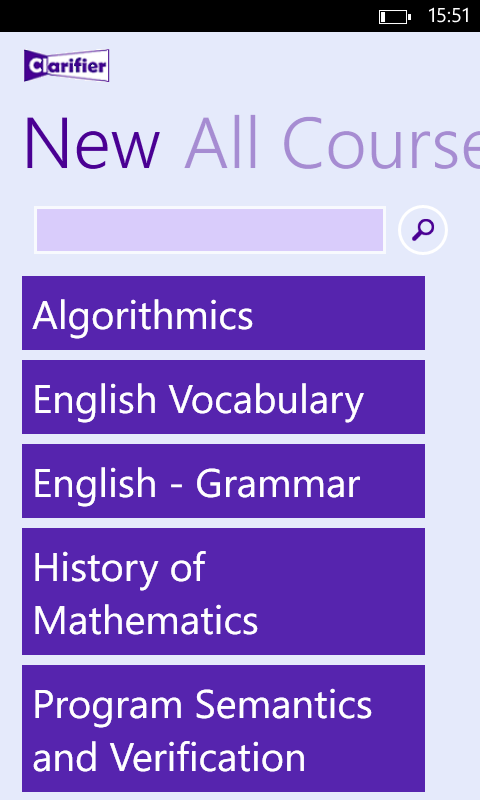
\includegraphics[width=0.4\textwidth]{Courses.png}
    \caption{Lista dostępnych przedmiotów}
    \label{fig:courses}
\end{figure}

Aby przejść do strony wybranego przedmiotu wystarczy nacisnąć kafelek z jego nazwą. W każdej zakładce możliwe jest również wyszukiwanie kursów po nazwie. W trybie offline po wybraniu w menu głównym opcji Downloads automatycznie otwiera się zakładka z listą pobranych przedmiotów i nie ma możliwości przejścia do innej zakładki. 

Po zalogowaniu na liście przedmiotów dostępna jest zakładka My Courses, która zawiera kursy dodane przez użytkownika do "moich kursów". W zakładce My Courses każdy kafelek z nazwą przedmiotu jest jednocześnie paskiem postępu informującym użytkownika, w jakim stopniu opanował materiał danego przedmiotu. 

\begin{figure}[t!]
    \centering
    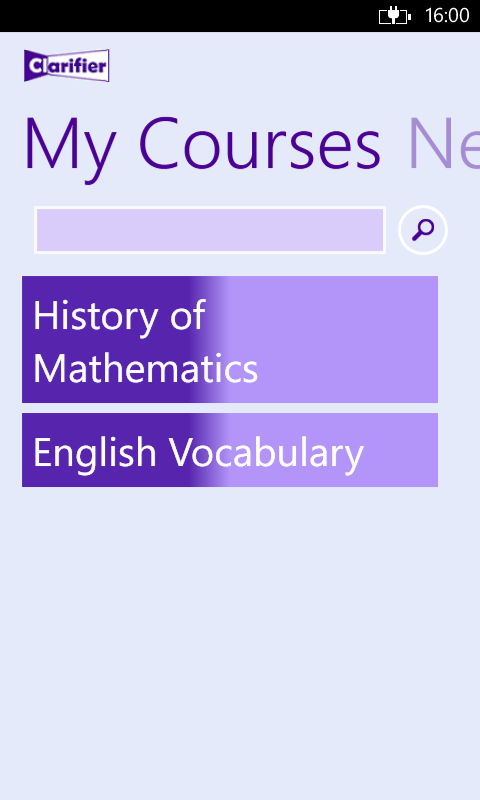
\includegraphics[width=0.4\textwidth]{Progress.png}
    \caption{Lista przedmiotów w zakładce My Courses}
    \label{fig:progress}
\end{figure}

\subsection{Strona przedmiotu}
Na stronie każdego przedmiotu znajduje się tytuł, krótki opis oraz lista dostępnych opcji. Menu kursu umożliwia rozpoczęcie powtórki w jednym z dostępnych trybów, zapisanie przedmiotu w pamięci telefonu, aktualizację pobranego wcześniej kursu oraz dodanie przedmiotu do "moich kursów".

Aplikacja oferuje następujące tryby powtarzania:
\begin{itemize}
\item Practice - tryb klasyczny; w tym trybie użytkownik otrzymuje kolejno wszystkie zadania z danego przedmiotu,
\item Study with Clarifier - tryb nauki kontrolowanej, dostępny tylko dla zalogowanych użytkowników,
\item 10Q Challenge - użytkownik otrzymuje dziesięć losowych pytań z danego przedmiotu,
\item Time Challenge - powtarzanie na czas; w tym trybie użytkownik ma za zadanie odpowiedzieć na jak najwięcej pytań w ustalonym czasie
\end{itemize}

\begin{figure}[h!]
    \centering
    
\includegraphics[width=0.4\textwidth]{Course.png}
    \caption{Strona przedmiotu}
    \label{fig:course}
\end{figure}

\newpage Tryb Study with Clarifier ułatwia użytkownikowi systematyczną naukę wybranego przedmiotu oraz kontrolę własnych postępów. W tym trybie zadania dobierane są według algorytmu, który uwzględnia poprzednio uzyskiwane wyniki oraz kolejność, w jakiej powinny być utrwalane moduły danego przedmiotu. W trakcie każdej powtórki użytkownik otrzymuje maksymalnie 18 pytań, w tym 10 losowych pytań z aktualnie przerabianego modułu oraz do 8 pytań z poprzednich modułów. Algorytm doboru zadań z poprzednich modułów wygląda następująco:
\newline
\newline
Niech $m$ - numer aktualnie przerabianego modułu (moduły indeksowane są od zera).
\newline Wówczas bazowa liczba pytań powtórkowych (tzn. pytań z już przerobionych modułów), jakie użytkownik otrzyma podczas najbliższej sesji powtórkowej wynosi:
\begin{center}
$p = 2m + 1 - [m=0]$, gdy $m < 4$
\end{center}
\begin{center}
$p = 8$, gdy $m >= 4$
\end{center}
Następnie dla każdego przerobionego modułu wyznaczamy dokładną liczbę pytań, jaka zostanie z niego wylosowana ($w_{i}$). Liczba pytań z danego modułu zależy od bazowej liczby pytań powtórkowych $p$ oraz liczby błędnie rozwiązanych zadań spośród ostatnich dziesięciu wykonanych zadań w danym module ($z_{i}$). Dla $i$-tego modułu liczbę zadań obliczamy ze wzoru
\begin{center}
$w_{i} = p * \frac{z_{i}}{\sum_{j=0}^m z_{j}}$
\end{center}
Wtedy łączna liczba pytań powtórkowych wynosi
\begin{center}
$u = \sum_{i=0}^m w_{i}$
\end{center}
Na wypadek gdyby uzyskana w ten sposób liczba pytań była mniejsza niż bazowa liczba pytań powtórkowych $p$, korygujemy uzyskany wynik zgodnie ze wzorem
\begin{center}
$P = u + [u<p]*(p-u)$,
\end{center}
gdzie $P$ - ostateczna liczba pytań powtórkowych, jakie użytkownik otrzyma podczas najbliższej sesji. Łączna liczba pytań, jaka zostanie przygotowana na najbliższą powtórkę wynosi
\begin{center}
$n = 10 + P$
\end{center}

\subsection{Moduły}
W przypadku trybów Practice, 10Q Challenge oraz Time Challenge, użytkownik zostanie poproszony o wybór modułów, które mają zostać objęte powtórką. Służy do tego lista modułów, która zostanie wyświetlona po wybraniu preferowanego trybu nauki na stronie przedmiotu. Możliwe jest zaznaczenie jednego, kilku lub wszystkich modułów przedmiotu.

\begin{figure}[h]
    \centering
    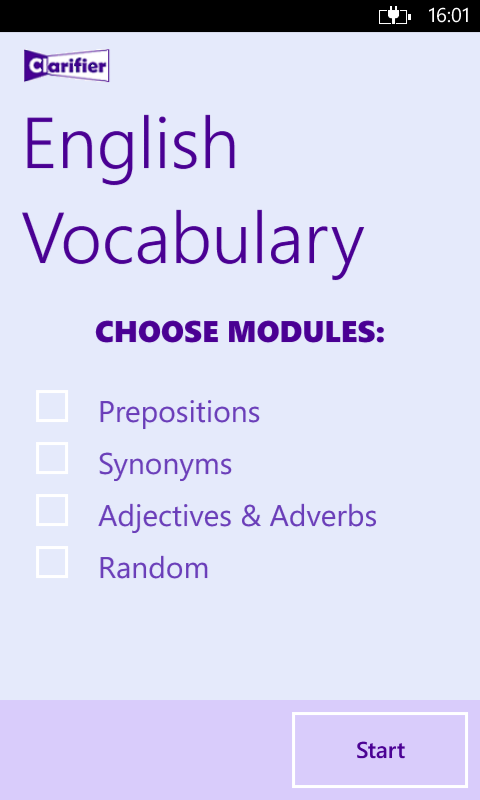
\includegraphics[width=0.4\textwidth]{Modules.png}
    \caption{Strona z listą modułów}
    \label{fig:modules}
\end{figure}

\subsection{Zadania utrwalające}
Po wybraniu jednego z trybów nauki na stronie przedmiotu oraz ew. modułów, które mają zosać objęte powtórką, na ekranie pojawi się pierwsze z przygotowanych zadań. Aplikacja Clarifier umożliwia rozwiązywanie zadań typu ABCD jedno- i wielokrotnego wyboru, zadań otwartych, gdzie poprawną odpowiedź należy wpisać w specjalnym polu tekstowym oraz zadań, w których użytkownik nie jest proszony o udzielenie odpowiedzi, a jedynie o zapoznanie się z treścią poprawnego rozwiązania. 

\begin{figure}[h]
    \centering
    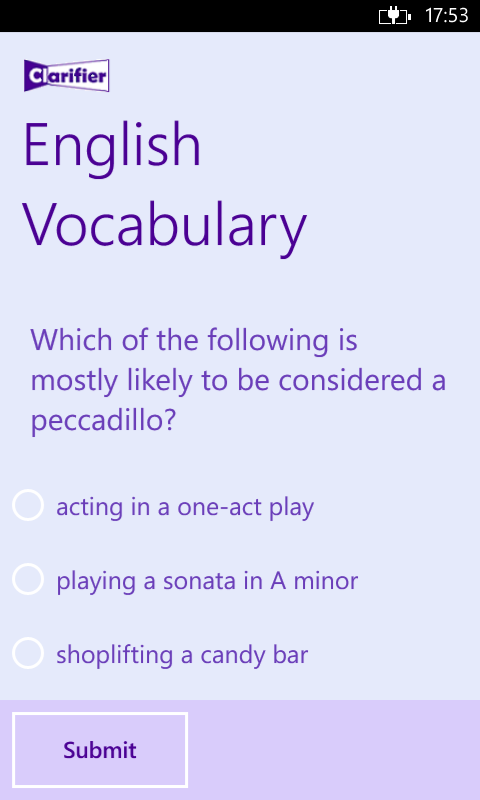
\includegraphics[width=0.3\textwidth]{Single_choice.png}
    \hspace{10.00mm}
    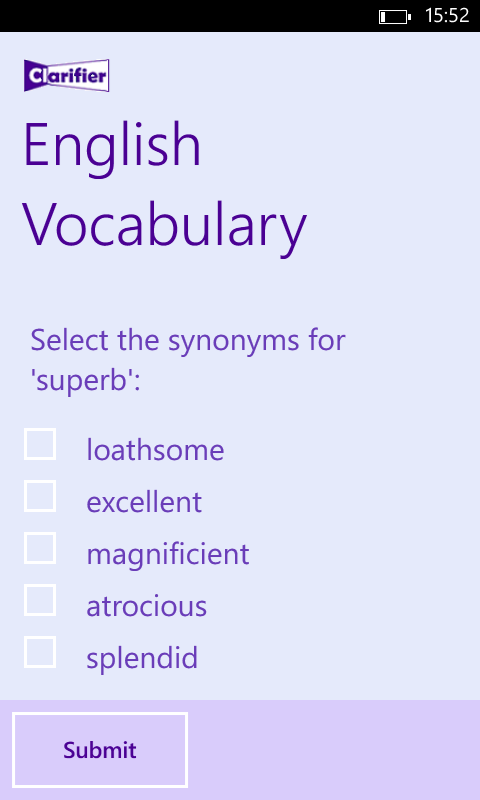
\includegraphics[width=0.3\textwidth]{Multiple_choice.png}
    \caption{Przykład zadania jedno- i wielokrotnego wyboru}
    \label{fig:exercise}
\end{figure}

Po wybraniu lub wpisaniu odpowiedzi, należy wcisnąć przycisk Submit. Na ekranie pojawi się wówczas komunikat informujący o tym, czy wprowadzona odpowiedź jest poprawna lub treść proponowanego rozwiązania w przypadku zadania, gdzie użytkownik nie był proszony o udzielenie własnej odpowiedzi. Aby przejść do następnego pytania wystarczy wcisnąć przycisk Next. Po rozwiązaniu ostatniego zadania na ekranie pojawi się podsumowanie wyników zakończonej sesji powtórkowej.

\begin{figure}[h]
    \centering
    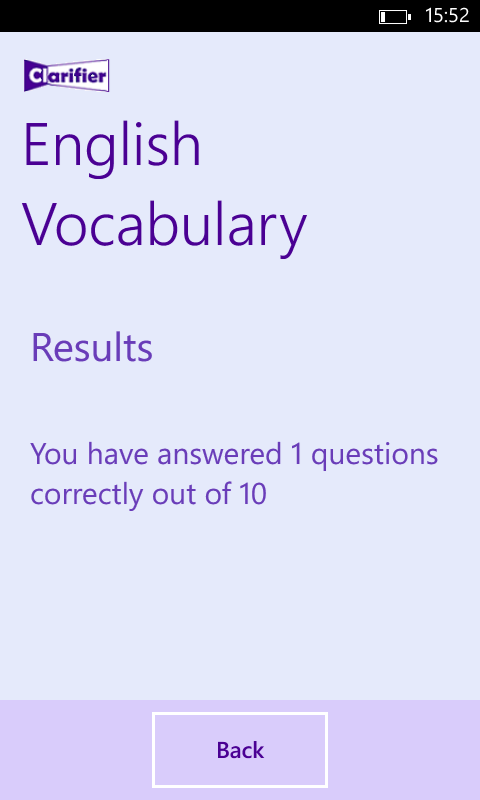
\includegraphics[width=0.3\textwidth]{Results.png}
    \caption{Podsumowanie wyników sesji powtórkowej}
    \label{fig:results}
\end{figure}

\section{Aplikacja webowa}

\chapter{Organizacja pracy}\label{r:org}

\section{Zakres}
Główną część pracy nad projektem Clarifier stanowiło zaprojektowanie i stworzenie opisanego w niniejszej pracy oprogramowania. Poza implementacją, prace nad projektem obejmowały tworzenie dokumentacji oraz przygotowywanie okresowych prezentacji na zajęcia z Zespołowego Projektu Programistycznego. 

\section{Zasoby}
Komunikacja pomiędzy członkami zespołu odbywała się za pośrednictwem mailowej grupy dyskusyjnej. Kod źródłowy oraz dokumentacja projektu były współdzielone za pomocą repozytorium systemu git.

\subsection{Dokumentacja projektu}
Dokumenty dotyczące projektu były tworzone za pomocą Google Docs. Prezentacje na zajęcia z Zespołowego Projektu Programistycznego były przygotowywane z wykorzystaniem Google Docs oraz serwisu \url{https://slides.com/}.

\subsection{Oprogramowanie}
Przy implementacji oprogramowania korzystaliśmy ze środowiska Microsoft Visual Studio 2013 oraz platformy Windows Azure. Do testowania aplikacji mobilnej wykorzystaliśmy telefony Nokia z systemem operacyjnym Windows 8.

\chapter{Podsumowanie}

\appendix

\chapter{Zawartość dysku CD}

\chapter{Podział pracy}

\begin{thebibliography}{99}
\addcontentsline{toc}{chapter}{Bibliografia}

\bibitem{Atkinson} R. C. Atkinson, R.M. Shiffrin, \textit{Chapter: Human memory: A proposed system and its control processes}, 1968, K.W. Spence, J.T. Spence, \textit{The psychology of learning and motivation (Volume 2)}, New York: Academic Press, s. 89–195.

\bibitem{Dudai} Dudai, Yadin, \textit{Memory from A to Z: Keywords, concepts, and beyond}, Oxford, UK: Oxford University Press, 2002.

\bibitem{Ebbinghaus} H. Ebbinghaus, \textit{Memory: A Contribution to Experimental Psychology}, \textit{Classics in the History of Psychology}, 1885-1913.

%\bibitem{Hebb} Hebb, O. Donald, "Distinctive features of learning in the higher animal", Delafresnaye, J. Francisque, \textit{Brain mechanisms and learning}, Oxford: Blackwell, 1961, s. 37–46.

\bibitem{Nikolic} D, Nikolić, W. Singer, \textit{Creation of visual long-term memory. Perception \& Psychophysics}, 2007.


\end{thebibliography}

\end{document}


%%% Local Variables:
%%% mode: latex
%%% TeX-master: t
%%% coding: latin-2
%%% End:
